\documentclass[12pt]{article}

\usepackage{report}

\usepackage[utf8]{inputenc} % allow utf-8 input
\usepackage[T1]{fontenc}    % use 8-bit T1 fonts
\usepackage[colorlinks=true, linkcolor=black, citecolor=blue, urlcolor=blue]{hyperref}       % hyperlinks
\usepackage{url}            % simple URL typesetting
\usepackage{booktabs}       % professional-quality tables
\usepackage{amsfonts}       % blackboard math symbols
\usepackage{nicefrac}       % compact symbols for 1/2, etc.
\usepackage{microtype}      % microtypography
\usepackage{lipsum}		% Can be removed after putting your text content
\usepackage{graphicx}
\usepackage{natbib}
\usepackage{doi}
\usepackage{listings}
\usepackage{xcolor}
\usepackage{float}
\setcitestyle{aysep={,}}



\title{Project Step 1}

\author{Brian Lee, Chloe Gentry, Vinny Rose\\
\AND\\
\AND
\AND
\AND
\AND
	CS.3339 Computer Architecture\\
\AND
	Texas State University\\
}

% Uncomment to remove the date
\date{September 25, 2024}

% Uncomment to override  the `A preprint' in the header
\renewcommand{\headeright}{Project Step 1 - Group Name}
\renewcommand{\undertitle}{Smarty Pants}
\renewcommand{\shorttitle}{}

\definecolor{codegreen}{rgb}{0,0.6,0}
\definecolor{codegray}{rgb}{0.5,0.5,0.5}
\definecolor{codepurple}{rgb}{0.58,0,0.82}
\definecolor{backcolour}{rgb}{0.95,0.95,0.92}

\lstdefinestyle{mystyle}{
    backgroundcolor=\color{backcolour},   
    commentstyle=\color{codegreen},
    keywordstyle=\color{magenta},
    numberstyle=\tiny\color{codegray},
    stringstyle=\color{codepurple},
    basicstyle=\ttfamily\footnotesize,
    breakatwhitespace=false,         
    breaklines=true,                 
    captionpos=b,                    
    keepspaces=true,                 
    numbers=left,                    
    numbersep=5pt,                  
    showspaces=false,                
    showstringspaces=false,
    showtabs=false,                  
    tabsize=2
}

\lstset{style=mystyle}


\begin{document}
\maketitle

\newpage
\tableofcontents
\thispagestyle{empty}


\newpage
\setcounter{page}{1}
\section{Introduction}
For step 1 we were assigned to design 4 computer circuits. A 1-bit Nand circuit, 1-bit Nor circuit, 1-bit Not circuit, and a 1x4 shifting circuit. We used Verilog to define the code for the circuits and GTKWave to simulate the waveforms for the circuits.

\section{1x4 Shift Circuit}
\label{sec:headings}

The 1x4 shift circuit takes a 4-bit input and shifts the bits to the left or right based on a control signal. This shifting operation moves each bit in the input to an adjacent position, with the vacant positions being filled by zeros. 

\subsection{Shift Circuit Verilog Code}
\lstinputlisting[language=Verilog]{1x4bit-shift/shift_tb.v}

To test the Shift circuit we have created 2 registers, one for the input and one for the shifting then one wire for the output. If this circuit works properly the output should display the input shifted to the left and zeros filling the shifted positions.
\lstinputlisting[language=Verilog]{1x4bit-shift/shift_tb.v}


\subsection{Shift Circuit Waveforms}

At 0 ns, we can see that A is 0, so the output Y is 0.
\begin{figure}[H]
    \centering
    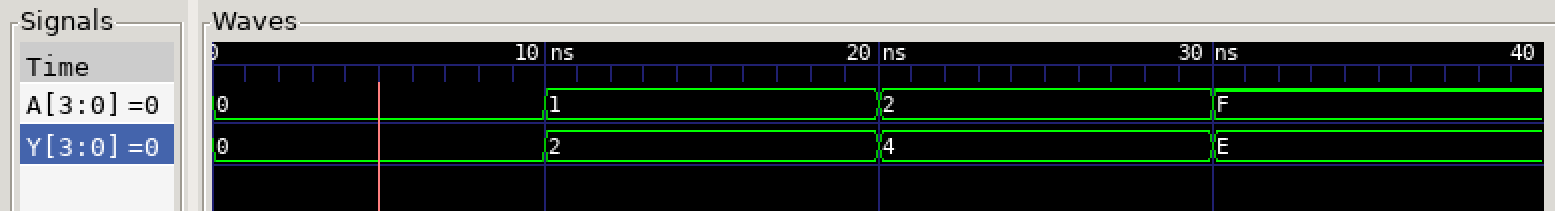
\includegraphics[width = 1.0\textwidth]{1x4bit-shift/shift_wave1.PNG}
    \caption{Shift Circuit with marker at 0ns}
    \label{fig:shift-wave1}
\end{figure}

At 10 ns, A is 1 (0001), so Y becomes 2 (0010).
\begin{figure}[H]
    \centering
    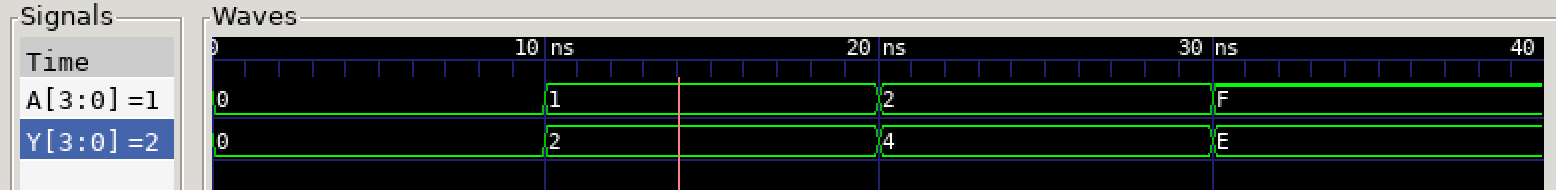
\includegraphics[width = 1.0\textwidth]{1x4bit-shift/shift_wave2.PNG}
    \caption{Shift Circuit with marker at 10ns}
    \label{fig:shift-wave2}
\end{figure}

At 20 ns, A is 2 (0010), so Y becomes 4 (0100).
\begin{figure}[H]
    \centering
    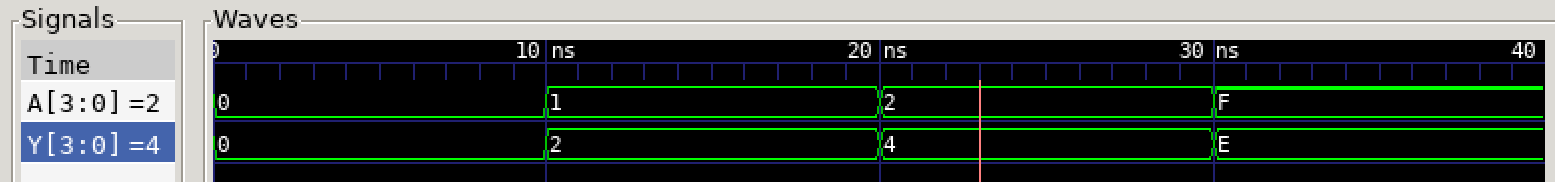
\includegraphics[width = 1.0\textwidth]{1x4bit-shift/shift_wave3.PNG}
    \caption{Shift Circuit with marker at 20ns}
    \label{fig:shift-wave3}
\end{figure}


At 30 ns, A is F (1111) so Y becomes E (1110).
\begin{figure}[H]
    \centering
    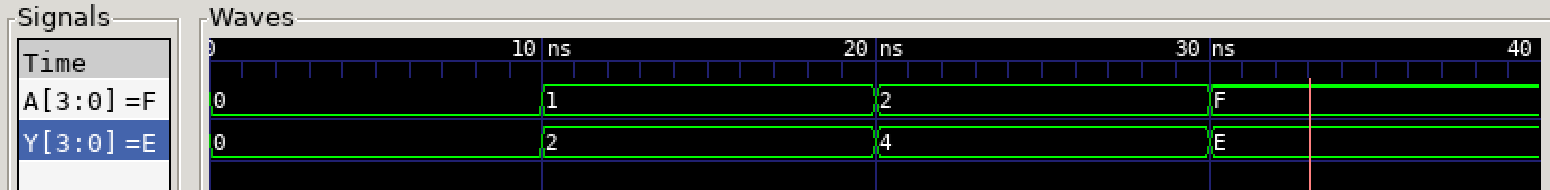
\includegraphics[width = 1.0\textwidth]{1x4bit-shift/shift_wave4.PNG}
    \caption{Shift Circuit with marker at 30ns}
    \label{fig:shift-wave4}
\end{figure}

\section{Not Circuit}
The Not circuit takes one input A, with an output Y. This will output a 0 if A is a 1, and will output 1 if A is a 0.

```\begin{figure}[H]
    \centering
    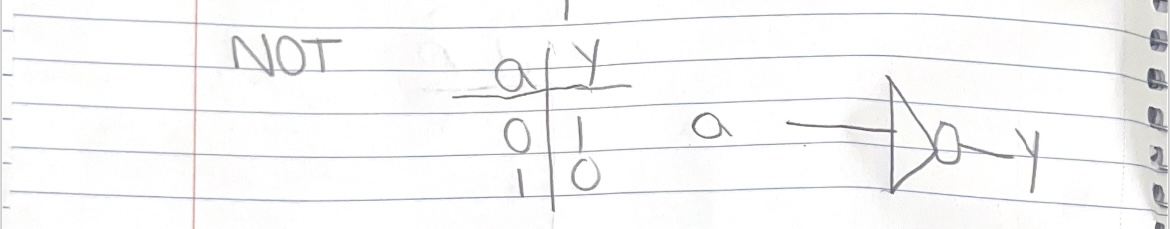
\includegraphics[width = 1.0\textwidth]{Truth-Tables/NotTT.PNG}
    \caption{Not truth table and gate}
    \label{fig:shift-table}
\end{figure}

\subsection{Not Circuit Verilog Code}
\lstinputlisting[language=Verilog]{not/not_gate.v}

To test the Not circuit, we have created one register A, as well as a wire Y. This way we are able to take each input for A and test output for A=0 and A=1. We'll know if this is working correctly if Y returns 1 for the test where A is 0 and Y returns 0 when A is 1.
\lstinputlisting[language=Verilog]{not/not_tb.v}

\subsection{Not Circuit Waveform}
At 2 ns, we can see that  A is 0, so the output Y is 1.
\begin{figure}[H]
    \centering
    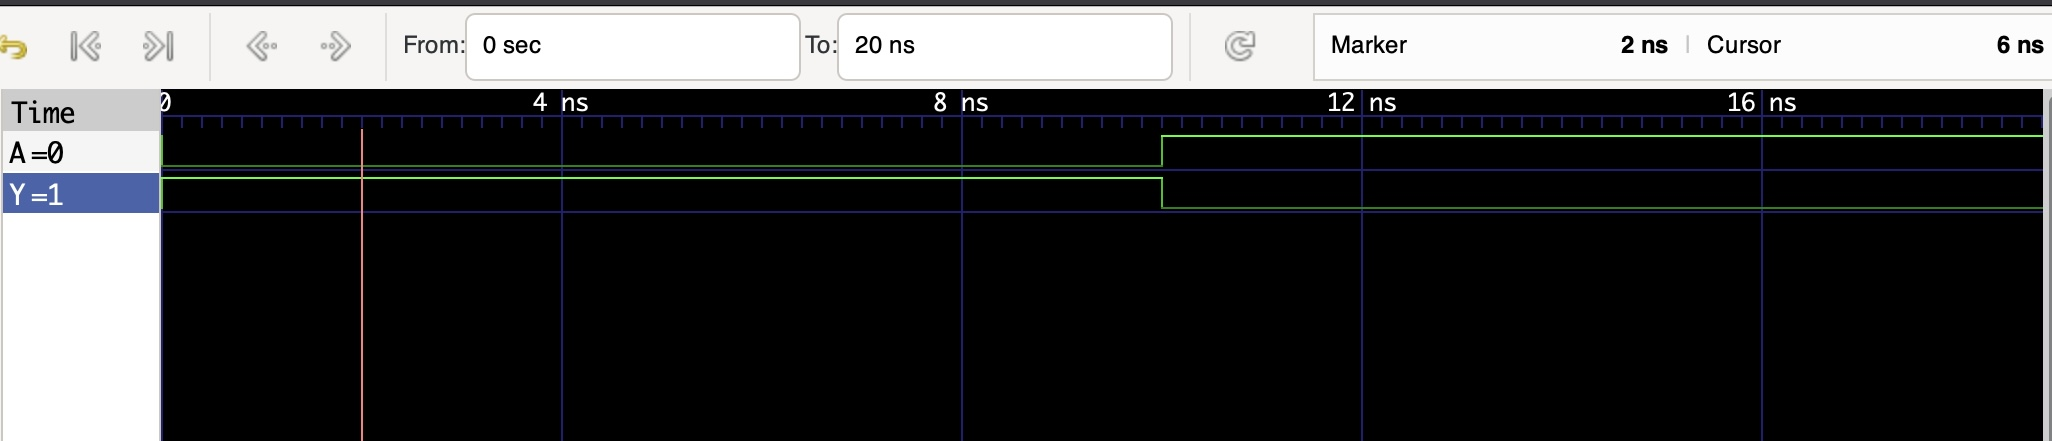
\includegraphics[width = 1.0\textwidth]{not/not_wave.PNG}
    \caption{Not Circuit with marker at 2ns}
    \label{fig:enter-label}
\end{figure}

At 10 ns, A becomes 1, so Y becomes 0.
\begin{figure}[H]
    \centering
    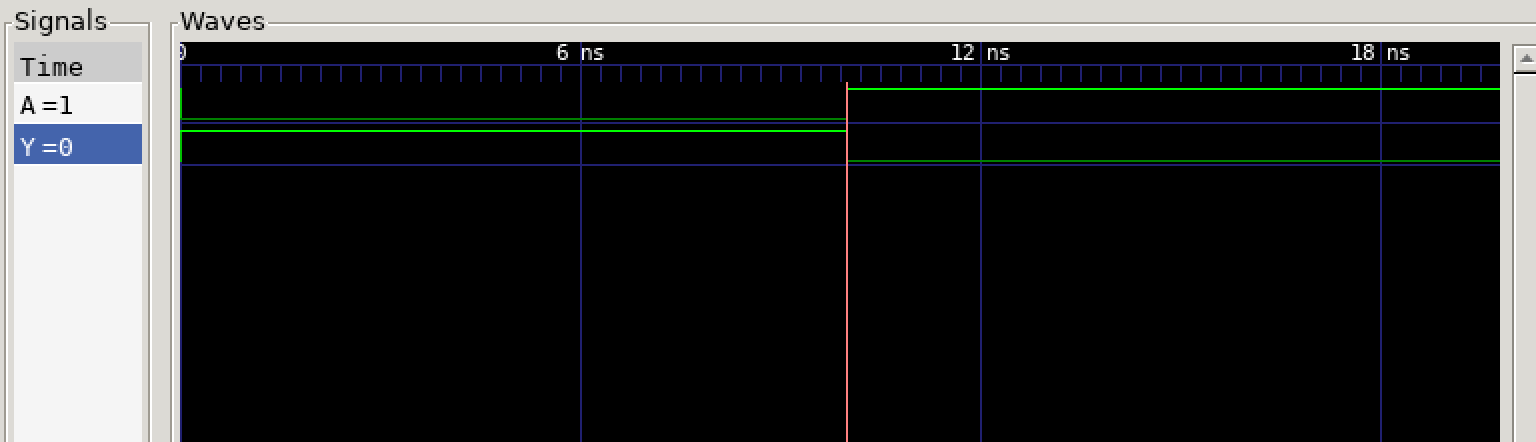
\includegraphics[width = 1.0\textwidth]{not/not_wave1.png}
    \caption{Not Circuit with marker at 10ns}
    \label{fig:enter-label}
\end{figure}

\section{Nand Circuit}
The Nand circuit takes two inputs, A and B, with an output Y. Nand will only give us back a 0 when A and B are both 1.

```\begin{figure}[H]
    \centering
    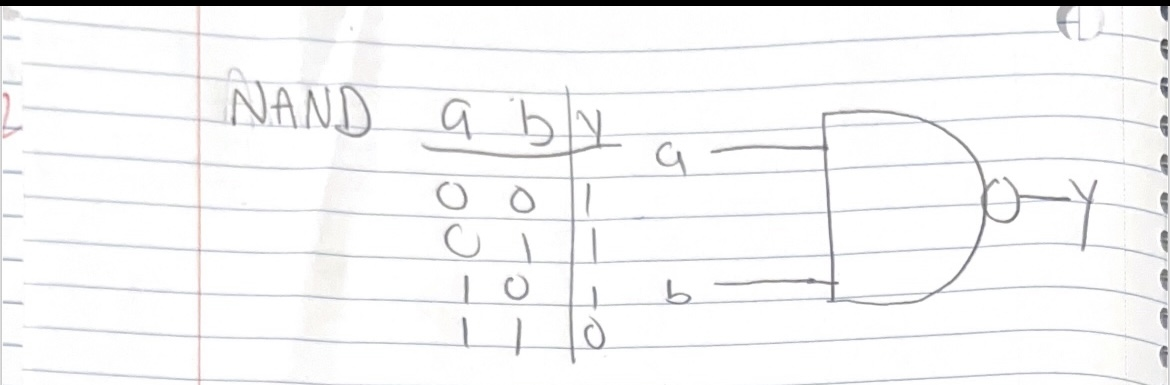
\includegraphics[width = 1.0\textwidth]{Truth-Tables/NandTT.PNG}
    \caption{Nand truth table and gate}
    \label{fig:shift-table}
\end{figure}

\subsection{Nand Circuit Verilog Code}
At 2 ns, we can see that  A is 0, so the output Y is 1.
\lstinputlisting[language=Verilog]{nand/nand_gate.v}

To test the Nand circuit, we have created two registers, A and B, as well as a wire Y. This allows us to test both inputs and one output. We'll know its correct if Y is 1 for all cases except where A and B are both 1.
\lstinputlisting[language=Verilog]{nand/nand_tb.v}
\subsection{Nand Circuit Waveform}

At 0 ns, A and B are 0, so Y is 1.
\begin{figure}[H]
    \centering
    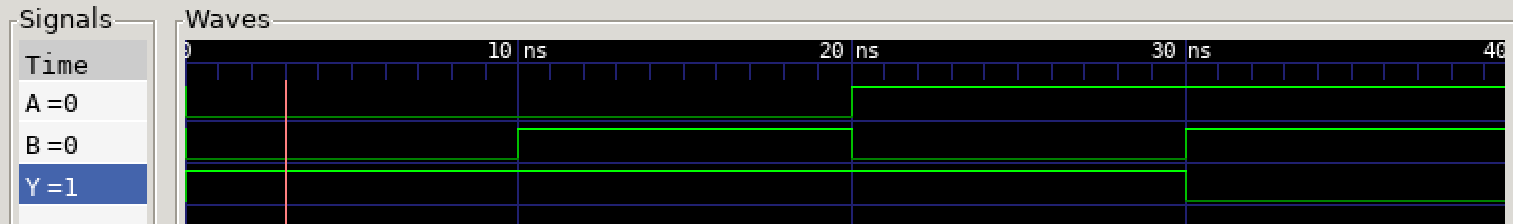
\includegraphics[width = 1.0\textwidth]{nand/nand_wave1.PNG}
    \caption{Nand Circuit with marker at 0ns}
    \label{fig:enter-label}
\end{figure}

At 10 ns, A is 0 and B is 1, so Y stays 1.
\begin{figure}[H]
    \centering
    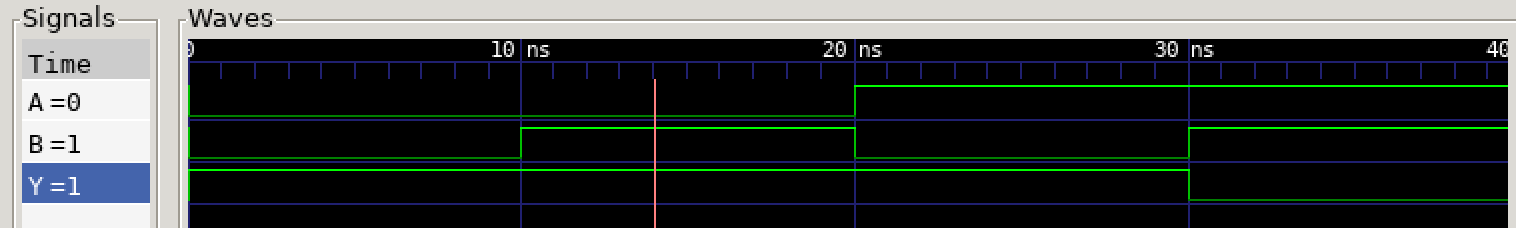
\includegraphics[width = 1.0\textwidth]{nand/nand_wave2.PNG}
    \caption{Nand Circuit with marker at 10ns}
    \label{fig:enter-label}
\end{figure}

At 20 ns, A is 1 and B is 0, so Y is still 1.
\begin{figure}[H]
    \centering
    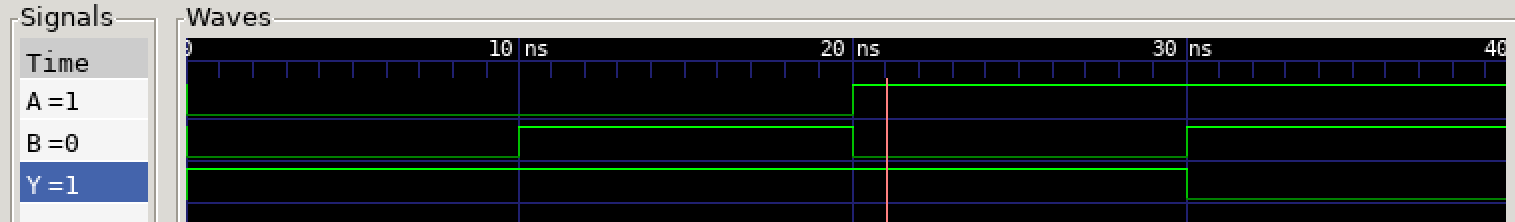
\includegraphics[width = 1.0\textwidth]{nand/nand_wave3.PNG}
    \caption{Nand Circuit with marker at 20ns}
    \label{fig:enter-label}
\end{figure}

At 30 ns, both A and B are 1, so Y finally flips to 0.
\begin{figure}[H]
    \centering
    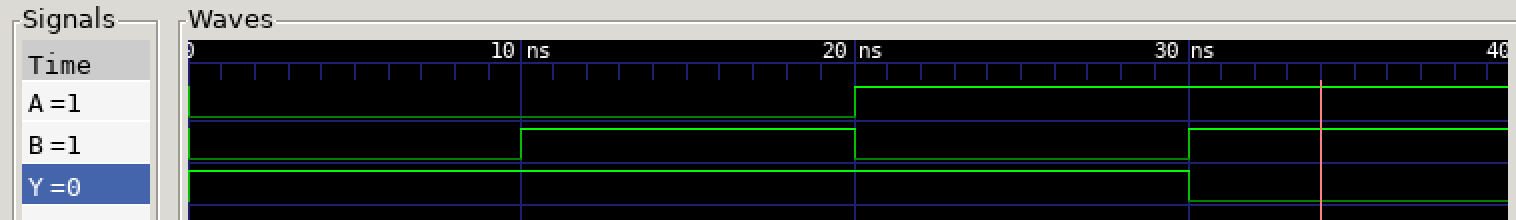
\includegraphics[width = 1.0\textwidth]{nand/nand_wave4.PNG}
    \caption{Nand Circuit with marker at 30ns}
    \label{fig:enter-label}
\end{figure}

\section{Nor Circuit}
The Nor circuit takes two inputs, A and B, with an output Y. This will output a 0 if either A or B is a 1, and will only output 1 if A and B are both 0.

```\begin{figure}[H]
    \centering
    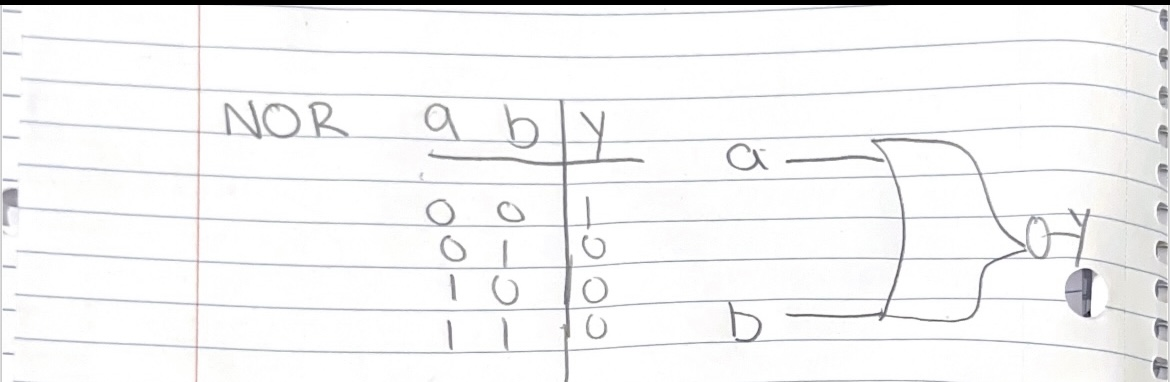
\includegraphics[width = 1.0\textwidth]{Truth-Tables/NorTT.PNG}
    \caption{Nor truth table and gate}
    \label{fig:shift-table}
\end{figure}

\subsection{Nor Circuit Verilog Code}
At 2 ns, we can see that  A is 0, so the output Y is 1.
\lstinputlisting[language=Verilog]{nor/nor_gate.v}

To test the Nor circuit, we have created two registers, A and B, as well as a wire Y. This way we are able to take two inputs at a time and test each possible input for the circuit. We'll know if this is working correctly if Y returns 1 for the test where A and B are 0 and Y should return 0 for the rest.
\lstinputlisting[language=Verilog]{nor/nor_tb.v}
\subsection{Nor Circuit Waveform}

At 0 ns, A and B are 0, so Y is 1.
\begin{figure}[H]
    \centering
    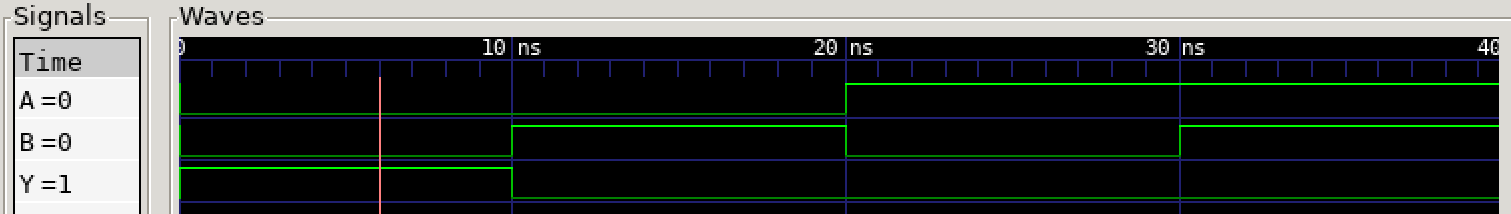
\includegraphics[width = 1.0\textwidth]{nor/nor_wave1.PNG}
    \caption{Nor Circuit with marker at 0ns}
    \label{fig:enter-label}
\end{figure}

At 10 ns, A is 0 and B is 1, so Y is now 0.
\begin{figure}[H]
    \centering
    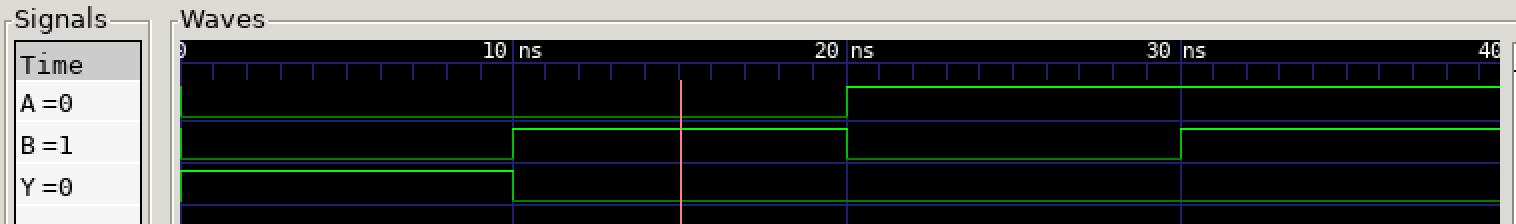
\includegraphics[width = 1.0\textwidth]{nor/nor_wave2.PNG}
    \caption{Nor Circuit with marker at 10ns}
    \label{fig:enter-label}
\end{figure}

At 20 ns, A is 1 and B is 0, so Y is still 0.
\begin{figure}[H]
    \centering
    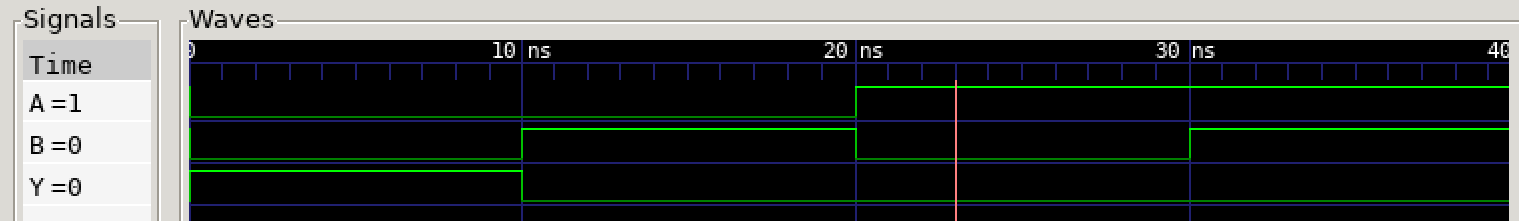
\includegraphics[width = 1.0\textwidth]{nor/nor_wave3.PNG}
    \caption{Nor Circuit with marker at 20ns}
    \label{fig:enter-label}
\end{figure}

At 30 ns, both A and B are 1, so Y again stays 0.
\begin{figure}[H]
    \centering
    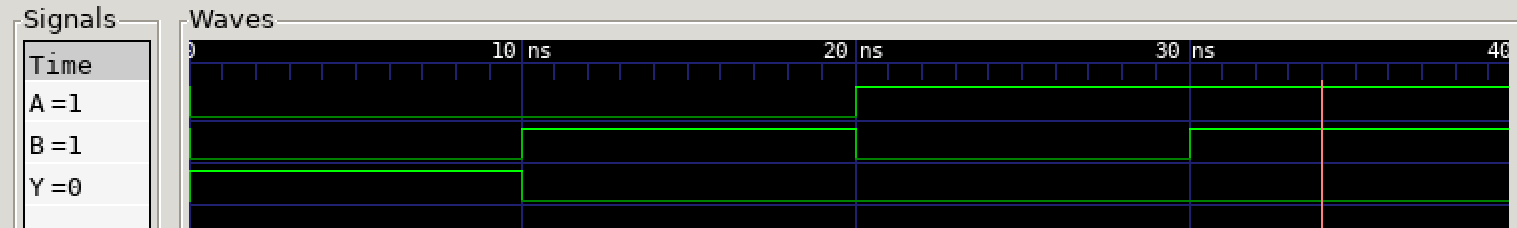
\includegraphics[width = 1.0\textwidth]{nor/nor_wave4.PNG}
    \caption{Nor Circuit with marker at 30ns}
    \label{fig:enter-label}
\end{figure}

\section{Conclusion}

In Conclusion, we created 4 different circuits in Verilog and simulated them in GTKWave. The logic was quite trivial but the biggest trouble we ran into was getting all of the software set up on our respective systems. We worked well together as a group and learned quite a bit about the basics of verilog and GTKWave.
\end{document}



